\documentclass[11pt,letterpaper]{article}
\usepackage{amsmath,graphicx,natbib}
\usepackage[top=2cm, bottom=2.5cm]{geometry}
\begin{document}
\title{GEO242 Final Project: How well can I image Owens Valley?}
\author{Ashley Stroup}
\maketitle


\section{Introduction}
\label{sec:Intro}

Plate tectonics is driven by mantle convection deep within the earth and is expressed most obviously at plate boundaries and fault systems at the surface. The major boundary types are convergent, divergent, and transform plate boundaries, however these systems often coevolve and transition between one another, influencing how oceanic crust and continental crust are formed, recycled, and deformed. Although the evolution and interaction of plate boundaries are well documented through geological and geodetic observations, many questions remain about the mechanisms responsible for the formation and evolution of plate boundaries. Many factors are thought to influence the evolution of plate boundary systems. The geologic history of a region is one of the important factors. Inherited weaknesses such as ancient sutures or shear zones and changes in lithology can guide the geometry of faults and strain partitioning in a plate boundary system  \citep[e.g.,][]{fang_new_2016, share_bimaterial_2018,schultepelkum_tectonic_2020}. Crustal thickness, magmatism, surface erosion, and sedimentation can all influence stress distribution and how plate boundaries reorganize over time \citep{wuinfluence_2021,long_evolution_2024}.

The San Andreas fault system is a modern example of a mature transform plate boundary, which evolved from a collision of a mid-oceanic rift with continental crust, due to subduction along the west coast of North America. The end of subduction has left uncertainty around how the subducted Farallon plate has influenced the tectonics and volcanism in the vicinity of the slab window. The present day plate boundary includes not only the mature San Andreas fault, but also a network of major faults which accommodate the transform plate motion between the Pacific Plate and North American plate (Figure~\ref{20percent}). 20-25 percent of the plate motion is accommodated in the Walker Lane and Eastern California Shear Zone (WL-ECSZ) \citep[e.g.,][]{dixon_constraints_1995, gan_strain_2000, miller_refined_2001, hammond_crustal_2007}. The WL-ECSZ incorporates strike-slip faulting east of the San Andreas, Sierra Nevada, and into parts of western Nevada. The WL-ECSZ is thought be organizing into a future inland plate-boundary jump \citep[e.g.,][]{faulds_kinematics_2005, faulds_tectonic_nodate, busby_birth_2013, stevens_structural_2013}.

\begin{figure}[!htbp]
    \begin{center}
        \includegraphics[width=10cm]{../Figures/20percent.png}
    \end{center}
    \caption{Map of the entire San Andreas fault system which accommodates the North America-Pacific plate motion \citep{Donnellan2017}.}
    \label{20percent}
\end{figure}

One area of particular interest in the WL-ECSZ is Owens Valley (Figure~\ref{OV_seismo_map}). Owens Valley is an extensional basin within the Basin and Range Province, which has moved the Sierra Nevada westward from the Colorado Plateau by a series of horst-graben or half-graben systems \citep{sonder_western_1999,hammond_block_2011}. Owens Valley is the westernmost basin, sandwiched between the highest point in the contiguous United States (Mt. Whitney) and the lowest point (Death Valley). The valley consists of two large basins, Bishop Basin and Owens Basin, which are separated by a structure arch at a latitude roughly coincident with the Poverty Hills, which are located south of Big Pine, CA \citep{hollett_geology_1991,danskin_evaluation_1998}. The northern boundary of Owens Valley is the Volcanic Tablelands/Round Valley/Chalfant Valley, transitioning into Long Valley. The southern boundary includes Owens Lake where the valley pinches out to become the much narrower Rose Valley and Coso Range. The broader region encompassing Owens Valley is labeled the Southern Walker Lane according to \citet{faulds_tectonic_nodate}. \citet{stevens_structural_2013} highlights that Owens Valley seems to be undergoing the early history of the Gulf of California and may become a rift valley as the plate boundary unzips northward. \textbf{This makes Owens Valley a prime candidate for studying not only its evolution into part of a mature transform plate boundary system, but also the transition into a divergent plate boundary system.}

\begin{figure}[!htbp]
    \begin{center}
        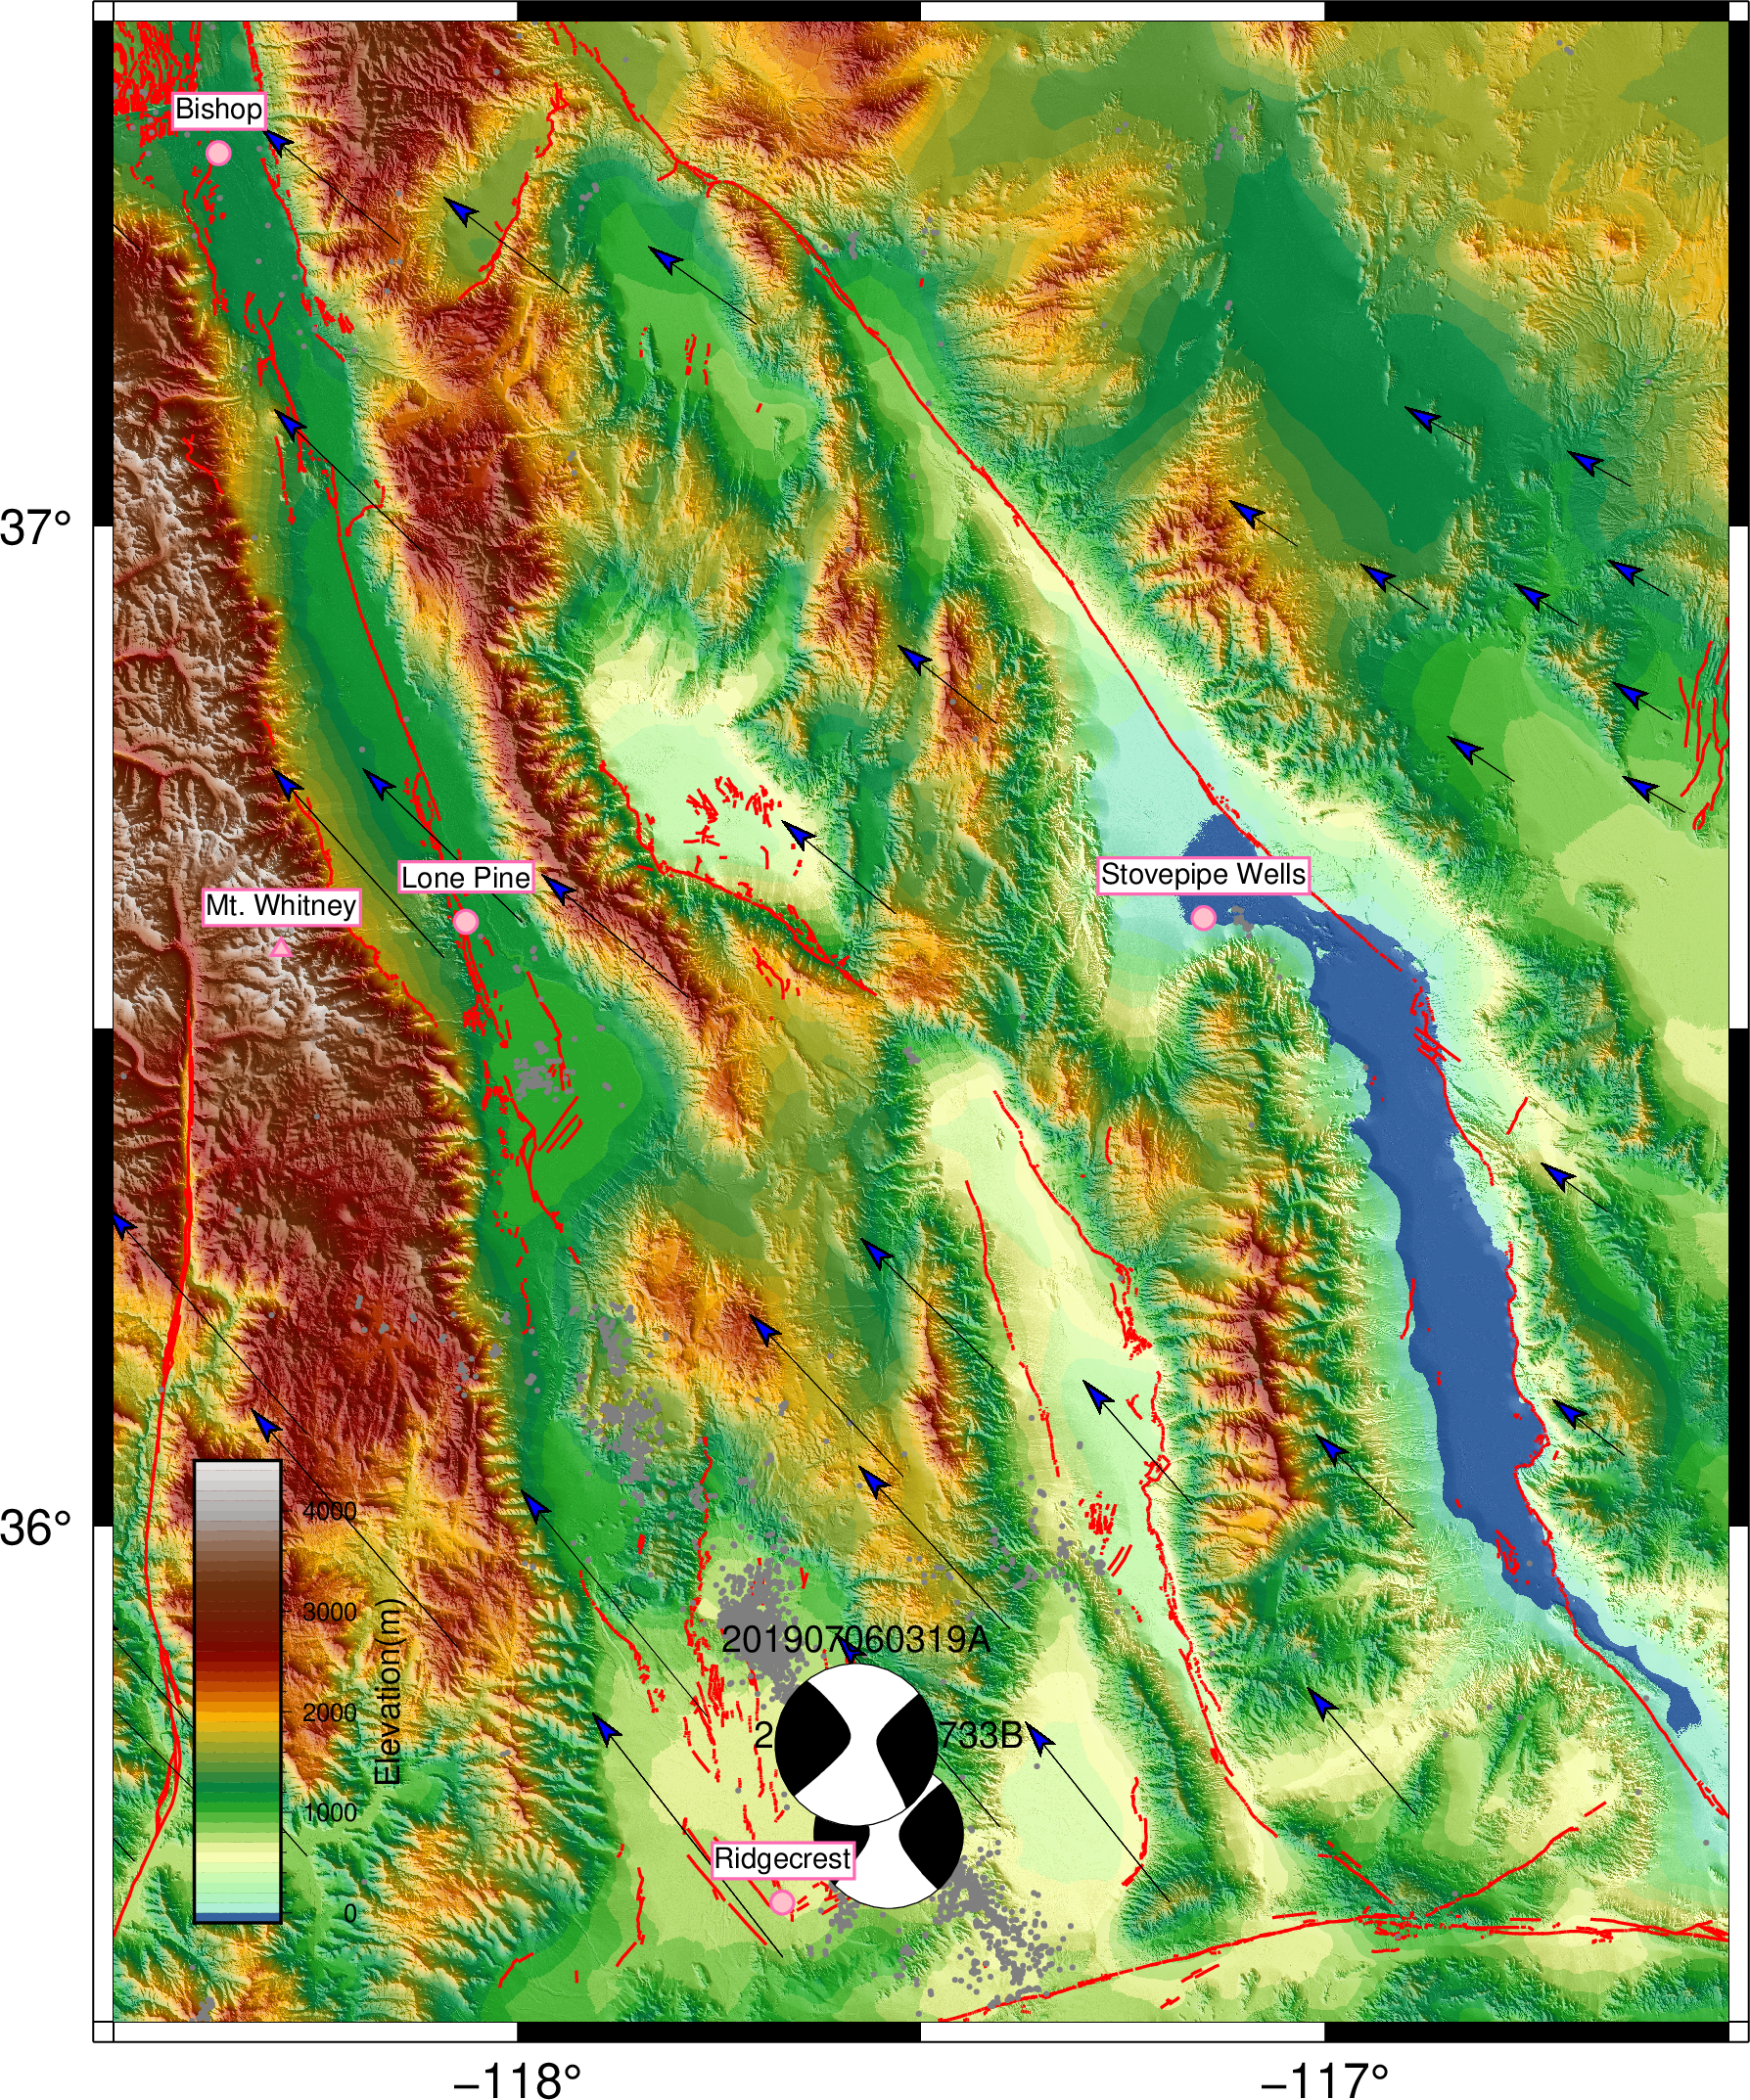
\includegraphics[width=10cm]{../Figures/OV_seismo_map.ps.png}
    \end{center}
    \caption{Map of Owens Valley (from south of Lone Pine to north of Bishop) with elevation, hillshade, seismicity (grey dots), faults (red lines), GPS velocities (arrows) and recent major earthquakes (beach balls). The pink circles represent major population centers and the pink triangles represent mountain peaks.}
    \label{OV_seismo_map}
\end{figure}

\section{Experiment}
\label{sec:Exp}

\subsection{Ambient Noise Tomography}
\label{sec:ANT}

Ambient noise tomography uses continuous seismic noise recorded by seismic station arrays to create shear wave velocity models of the crust and uppermost mantle \citep{shapiro_high-resolution_2005,lin_complex_2011,wang_ambient_2019,lee_imaging_2025}. The sources of the noise can be due to oceanic microseisms, atmospheric processes, or anthropogenic activity \citep{yang_characteristics_2008,schwardt_natural_2022}. Cross-correlations of the noise between station pairs allows Green’s functions to be extracted. These Green’s functions are then used to generate surface wave dispersion curves which can then be inverted to produce shear velocity models \citep{bensen_processing_2007,lin_eikonal_2009,luo_limitations_2015}. Other methods, like Rayleigh wave ellipticity, earthquake tomography, and receiver functions, can then be jointly inverted to improve the velocity model \citep[e.g.,][]{li_joint_2019, berg_shear_2020}. As in all surface wave imaging studies, short-period waves are more sensitive to shallow structure, while long-period waves are more sensitive to deeper structures. 

The ambient noise method is a popular passive source imaging method because it does not require large magnitude teleseismic earthquake arrivals, but instead leverages ambient noise, allowing for shorter deployments of instruments given sufficient noise. Multiple studies use this method to image crustal and upper mantle structure in places such as California \citep{lin_high-resolution_2013,wang_refined_2018}, Alaska \citep{berg_shear_2020}, and Haiti \citep{lee_imaging_2025}. The studies target different resolutions and depths dependent on how the arrays are configured. For example, \citet{lin_3-d_2014} used the EarthScope Transportable Array (70 km station spacing) to create a model of the entire western U.S. from 1 km to 80 km depth, while \citet{wang_imaging_2019} deployed 71 geophones along a ~1km line to image the damage zone on a strand of the San Jacinto fault. 

In our proposed analysis, we will follow the temporal normalization and spectral whitening procedures outlined in \citet{bensen_processing_2007} and \citet{lin_3-d_2014} to prepare the three-component data from all stations. The horizontal components will be rotated from east-west and north-south to radial and transverse components before cross-correlating all station-pairs following \citet{lin_2008}. We will improve the signal-to-noise ratio (SNR) by summing the positive and negative components of each cross-correlation \citep{wang_ambient_2017}. Station pairs will use combinations of vertical (Z) and radial (R) components, ZZ, ZR, RZ, and RR, to calculate Rayleigh wave phase velocities. When array design permits, we will also calculate horizontal-versus-vertical (H/V) amplitude ratios to jointly invert with the phase velocities. To determine the phase velocities and amplitudes, we will apply frequency-time analysis (FTAN) as described in \citet{bensen_processing_2007}. We will invert the phase velocities using the tomographic method of \citet{barmin_fast_2001} for a 2-D Rayleigh wave phase velocity map. At each station, we will jointly invert the phase velocities and H/V ratios to create a 1-D shear velocity model using the Markov Chain Monte Carlo (MCMC) method \citep{berg_shear_2020,liu_highresolution_2021}. These models will be combined to create 2-D and 3-D tomographic models for Owens Valley, dependent on the array design used, which we discuss in more detail in our section on array design. 

\subsection{Challenges}
\label{sec:Challenges}

The research plan for this proposal is centered on a seismic deployment within Owens Valley. The deployment will consist of a mixed mode, passive source seismic imaging experiment of both Bishop Basin and Owens Basin. However, such a deployment faces multiple logistical challenges. First, the majority of the land is public land owned and managed by the Los Angeles Department of Water and Power (LADWP), Bureau of Land Management (BLM), and the U.S. Forest Service (USFS). A second challenge is that accessibility is uneven, with significant portions of the valley being inaccessible (no roads) or marginally accessible (roads requiring high clearance 4x4). To address these issues as best as possible, we have completed five trips to the valley to survey road conditions. The trips allowed us to survey road hazards, confirm accessibility for 4x4 vehicles, and create a map of locations suitable for station deployment, all in order to begin permitting. Since the road condition mapping has been completed, we have been in contact with the public landowners to complete permitting. 

The second major logistical limitation of our proposed work is the narrowness of Owens Valley, which is surrounded by steep mountain slopes, meaning there is limited accessibility outside of the valley. As a result, there are issues making the experiment’s aperture wide enough to image basin structure for ambient noise tomography. We plan to address this limitation by including permanent broadbands within and surrounding the valley and deploying our own temporary broadband stations along key mountain access points. The broadband components are necessary to increase aperture width, which is essential for ensuring that source-receiver pairs in ambient noise tomography are far enough apart \citep{luo_limitations_2015} to constrain structure to sufficient depths.

Based on the limitations described above, and considering the scientific goals of this proposal, we have designed an array that can be broken up into two parts: (1) 32 broadband stations deployed within, and outside of, the valley (Figure~\ref{stations}a). (2) A 2D nodal array of 175 stations with 4 km spacing will be deployed within the valley, allowing for higher resolution coverage of the two basins and Big Pine Volcanic Field (Figure~\ref{stations}b). Below, we provide a detailed description of each array type, including duration, the scientific target(s) of each array, and any notable limitations or challenges we anticipate.  

\begin{figure}[!htbp]
    \begin{center}
        \includegraphics[width=12cm]{../Figures/stations}
    \end{center}
    \caption{(a) Map of existing broadband network (purple) and our proposed broadband network (green). (b) Map of the nodal deployment (red). Blue lines are high density nodal deployments not within the scope of this project.}
    \label{stations}
\end{figure}

\subsection{Array Designs}
\label{sec:Array}

\subsubsection{Broadband Deployment}
\label{sec:BB}

The backbone of our experiment involves the deployment of about 32 broadband stations, which will be deployed for two years (Figure~\ref{stations}a). By installing broadbands in the Sierra Nevada and White-Inyo Mountains we will be able to increase the aperture of the nodal experiment by ~5-10 km, which is essential for the ambient noise tomography method as it requires at least three wavelengths between station pairs \citep{bensen_processing_2007}, although some workers have opted to use less restrictive criteria \citep{luo_limitations_2015,wang_ambient_2017} and is something we may pursue. While it would be hypothetically appropriate to instrument these mountain locations with additional nodal seismometers that would collect data for 30 days, broadband data collected over a two-year period of time can be used to address a broader set of science questions than nodal seismometers alone. By combining data from the temporary broadband array along with the 45 permanent stations in the region, we can generate an ambient noise tomography model with deeper resolution across the entire southern Walker Lane region, and not just Owens Valley.

\subsubsection{Nodal Deployment}
\label{sec:Node}

Our second major field effort will be the deployment of 175 nodal seismometers with 4 km spacing within Owens Valley (Figure~\ref{stations}b). The nodes will be deployed for 30 days, which is based on their battery life. Jointly inverting both phase velocities and H/V ratios will provide higher resolution from within the first kilometer and down \citep{berg_shear_2020}. The data from the 2D nodal array will allow us to create a 3-D model of Owens Valley to address the presence of melt and seismic hazard estimates for the valley. The data available for seismic hazard assessment is far from comprehensive. The SCEC community velocity model \citep[CVM-S4.26,][]{lee_full3d_2014} model does not have great agreement with the models from the \citet{pakiser_structural_1964} and \citet{stevens_structural_2013}. The major population center in the region, Bishop, sits on a basin of unknown depth, shape, or mapped subsurface faults. There is also extensive water infrastructure and agriculture for the state that needs better seismic hazard assessments to best mitigate damage in the event of a large earthquake. The 2D nodal array will increase the resolution within the valley to better constrain the fault and basin structure which the broadband array cannot provide with its larger spacing.

\section{How well can I image the valley?}
\label{sec:well}

For the final project for GEO242, we were challenging to use many of the skills we have learned in class to address something around our own research. As described in Section~\ref{sec:Exp}, I am attempting to do a massive seismic deployment in Owens Valley. This begins as my qualifying proposal, however, my hope is to submit the proposal to one or both the USGS and NSF to obtain funding for this massive deployment. In order to do that, I need to calculate how well I will be able to image the valley using these two deployment as justification. This proposed the perfect problem to address for my final project! I created a code (1) extract the station coordinates and plot the stations, (2) plot all of the possible station pairs and obtain the longest and shortest distances between those station pairs, (3) calculate the peak sensitivity, depth sensitivity, lateral resolution, and vertical resolution.

\subsection{Plotting the stations}
\label{sec:plot}

First challenge I needed to handle to start this was to simply get the latitude and longitude of each station. These were originally plotted in CalTopo, which does not have a way of downloading simply the coordinates. It can create a .kml file, but that was not in the same format as we had used in class and proved to not be very useful. I ended up uploading the .kml file to Google Earth and downloading a new (and familiar) .kml file from there. Then I was able to extract all the coordinates from the .kml file to begin using in my maps. I was able to make heavy use of the maps we originally made in calss to show seismiscity in a region. Figure~\ref{bb deployment} show the both temporary and permanent broadband stations and Figure~\ref{node deployment} displays the ~175 nodal deployment within the valley.

\begin{figure}[!htbp]
    \begin{center}
        \includegraphics[width=12cm]{../broadband_map.ps.png}
    \end{center}
    \caption{Map of Owens Valley with the temporary and permentant broadbands described in Section~\ref{sec:BB} as blue dots, approximately 32 temporary deployments (primarly concentrated within the valley) and 45 existing network stations}
    \label{bb deployment}
\end{figure}

\begin{figure}[!htbp]
    \begin{center}
        \includegraphics[width=6cm]{../nodes_map.ps.png}
    \end{center}
    \caption{Map of Owens Valley with the nodal deployment described in Section~\ref{sec:Node} as blue dots, approximately 175 stations}
    \label{node deployment}
\end{figure}

\subsection{Distances Between Stations}
\label{sec:distances}

The next challenge was figuring out the longest and shortest distances between station pairs. This is important to ambient noise tomography because this is what determines the limits of your imaging capabilities in an experiment. As mentioned in Section~\ref{sec:BB}, the method relies on having three wavelengths between stations to determine how deep you can image with the array \citep{bensen_processing_2007}. Therefore, its advantagous to get as wide of an aperture as possible to see as deep as possible, mentioned in Section~\ref{sec:Challenges}. The shallowest we can see is determined by the shortest spacing between stations. In order to determine these values, I wanted to plot all possible combinations. This would give us an idea of our coverage across and around the valley while also recording all possible station pairs to determine our longest and shortest distances. My code plots two different plots, one of just all possible station pairs and another with the longest and shortest distances. I have included the longest and shortest distance plots (Figure~\ref{bblimit} and Figure~\ref{nodelimit}) here to avoid having nearly redundant figures. In order to get these distances, I had to use the Haversine formula (Equation~\ref{haversine}) which uses the coordinates to calculate the distance into distance.

\begin{equation}
\begin{aligned}
    a &= \sin^2\left( {\frac{\phi_2-\phi_1}{2}} \right)+\cos{\phi_1}\cos{\phi_2}\sin^2\left( {\frac{\lambda_2-\lambda_1}{2}} \right) \\
    c &= 2 \arcsin(\sqrt{a}) \\
    d &= Rc
    \label{haversine}
\end{aligned}
\end{equation}

In Equation~\ref{haversine}, $a$ calculates the haversine of the central angle between two points, $c$ is the angle in radians between two points, and $d$ calculates the distances on a sphere, in this case, Earth with a radius of 6371 kilometers. $\phi$ are the latitude of two points, $\lambda$ are the longitude of two points.

\begin{figure}[!htbp]
    \begin{center}
        \includegraphics[width=12cm]{../broadband_limit_map.ps.png}
    \end{center}
    \caption{Map of Owens Valley with the all possible station pairs between broadbands (light blue), longest distance (269 km, magenta), and shortest distance (0.6 km, green).}
    \label{bblimit}
\end{figure}

\begin{figure}[!htbp]
    \begin{center}
        \includegraphics[width=6cm]{../nodes_limit_map.ps.png}
    \end{center}
    \caption{Map of Owens Valley with the all possible station pairs between nodes (light blue), longest distance (142 km, magenta), and shortest distance (1.7 km, green).}
    \label{nodelimit}
\end{figure}

\subsection{Sensitivity Calculations}
\label{sec:calc}

Once I have obtained the distances from both arrays, the next step was calculating the estimated sensitivies, or limits as I called them. I did need a initial estimate for the crustal velocity in the region, so I took an average of values in \citet{pakiser_structural_1964}, which gave me approximately 2.6 kilometers per second to run these estimates. For the shallowest sensitivity, I used Equation~\ref{shallow}. It calculates the shortest wavelength we can use in our experiment, which is two times the shortest station spacing. To calculate the deepest sensitivity, three wavelengths are required between the longest station pairs, calculated using Equation~\ref{deep}. For both arrays, I also calculated the highest or lowest frequencies and converted those to period using Equations~\ref{fp}.

\begin{equation}
        \lambda = 2(d_s)
        \label{shallow}
\end{equation}

\begin{equation}
    \lambda = \frac{d_l}{3}
    \label{deep}
\end{equation}

\begin{equation}
    \begin{aligned}
        f = \frac{v}{\lambda} \\
        p = \frac{1}{f}
        \label{fp}
 \end{aligned}
\end{equation}

In these equations, $\lambda$ is wavelength, $d_s$ is the shortest distance, $d_l$ is the longest distance, $v$ is the \citet{pakiser_structural_1964} velocity, $f$ is frequency, and $p$ is the period. The wavelengths calculated in Equation~\ref{shallow} and Equation~\ref{deep} are the critical number needed to calculate the sensitivity limits for the experiment. The three equations needed for these calulcations are listed below:

\begin{equation}
    d_\text{peak} = \left( {\frac{1}{3}} \right)\lambda
    \label{peak}
\end{equation}

\begin{equation}
    d_\text{lateral} = \left( {\frac{1}{2}} \right)\lambda
    \label{lateral}
\end{equation}

\begin{equation}
    d_\text{vertical} = \left( {\frac{1}{4}} \right)\lambda
    \label{vertical}
\end{equation}

In these equations, $d$ is the depth in kilometers and $\lambda$ is the wavelength. Equation~\ref{peak} calulcates the peak sensitivity, which is where we will have the best resolution. Equation~\ref{lateral} calculates the lateral sensitvity or how small of a feature we can resolve. This calculation also gives us the depth senstivity which is the maximum depth we hope to have resolution to. Equation~\ref{vertical} calculates the vertical resolution or how small of a layer can be vertically for us to resolve. Each one of these calulcation gives us an estimate for how deep we see and what types of features we can hope to resolve. The results for the broadbands are in Table~\ref{tab:BB} and the nodal array results are in Table~\ref{tab:node}.

\begin{table}[h!]
    \caption{Broadband results with from calculations in Equations~\ref{peak}, \ref{lateral}, and \ref{vertical}. The shallow limits are listed first, followed by the deep limits. These measurements are in kilometers.}
    \begin{center}
        \begin{tabular}{|c|c|c|c|}
        \hline
        \multicolumn{4}{|c|}{Broadband Array} \\
        \hline
        \multicolumn{4}{|c|}{Shallow Limits (km)} \\
        \hline
        Peak & Depth & Lateral & Vertical \\
        \hline
        0.4 & 0.6 & 0.3 & 0.6 \\
        \hline
        \multicolumn{4}{|c|}{Deep Limits (km)} \\
        \hline
        Peak & Depth & Lateral & Vertical \\
        \hline
        29.9 & 44.9 & 22.9 & 44.9 \\
        \hline
        \end{tabular}
    \end{center}
    \label{tab:BB}
\end{table}

\begin{table}[h!]
    \caption{Nodal results with from calculations in Equations~\ref{peak}, \ref{lateral}, and \ref{vertical}. The shallow limits are listed first, followed by the deep limits. These measurements are in kilometers.}
    \begin{center}
        \begin{tabular}{|c|c|c|c|}
        \hline
        \multicolumn{4}{|c|}{Nodal Array} \\
        \hline
        \multicolumn{4}{|c|}{Shallow Limits (km)} \\
        \hline
        Peak & Depth & Lateral & Vertical \\
        \hline
        1.2 & 1.7 & 0.9 & 1.7 \\
        \hline
        \multicolumn{4}{|c|}{Deep Limits (km)} \\
        \hline
        Peak & Depth & Lateral & Vertical \\
        \hline
        15.8 & 23.7 & 11.8 & 23.7 \\
        \hline
        \end{tabular}
    \end{center}
    \label{tab:node}
\end{table}

\subsection{Conclusions and Future Improvements}
\label{sec:improve}

Honestly, these results were pretty eye opening. It seems that we have much better coverage than I first suspected, in both the density of lines seen in Figure~\ref{bblimit} and \ref{nodelimit} and the depths we might be able to image with both arrays seen in Table~\ref{tab:BB} and \ref{tab:node}. The nodal array should be able reach up to 18 second periods while the broadband array should reach up to 35 second periods! Given the concerns mentioned in Section~\ref{sec:Challenges}, especially the narrow nature of Owens Valley, I am happy with the coverage. The results from the study will be on two scales: locally in Owens Valley and regionally in southern Walker Lane. These estimates are also the "worst case" scenarios if we cannot get the less constrictive criteria to work like mentioned in Section~\ref{sec:BB}.

Although I am happy with my effort here, I want to acknowledge some ways I'd like to improve this code for future use. There are some bigger picture goals like simply clenaing up the code to run on one dataset at a time to make it more user friendly or cleaning up some of the math with functions. However, the areas that concern me most are with the shallow limits. Highlighted in Figure~\ref{bblimit} and \ref{nodelimit}, the shortest distances are too small to be an average value of the larger dataset. Especially in the nodal dataset where our goal was to plot the stations with ~4 km spacing, so the 1.7 km shortest distance is not representative. Ultimately, for both datasets, the shortest distance is much too local of a measure to get an accurate value for our shallow limits. This could be relatively easily remedied with put a "larger than or equal to" clause, but I do think I could more qualitatively find an average small value in future iterations. Additionally, it would be nice to find the longest distances between stations quasi-parallel and perpendicular to the valley itself to include additional estimates in future iterations. Perhaps I can do something similar to how Gareth found the distances from the stations to the San Andreas fault, I'm not sure, I'd have to think about it. The most intimidating goal would be to create a 3D model of the limits with resolution coverage for the experiment, however I am not confident enough in my abilities to achieve that with this class.

Ultimately, I am really proud of myself for accomplishing the code and the report in LaTex. I went into this with a sense of dread because I remember struggling so much with coding in Roby's Python class and the theories behind my research with no geophysical background. However, I have learned a lot since my first few quarters here and I was able to create this code and write this without many crash-outs. Here's to hopefully putting instruments in the ground in 2026!
    
\bibliographystyle{apa-good}
\bibliography{final_project_bib}


\end{document}
